\documentclass[12pt,letterpaper]{article}
\usepackage{graphicx,textcomp}
\usepackage{natbib}
\usepackage{setspace}
\usepackage{fullpage}
\usepackage{color}
\usepackage[reqno]{amsmath}
\usepackage{amsthm}
\usepackage{fancyvrb}
\usepackage{amssymb,enumerate}
\usepackage[all]{xy}
\usepackage{endnotes}
\usepackage{lscape}
\newtheorem{com}{Comment}
\usepackage{float}
\usepackage{hyperref}
\newtheorem{lem} {Lemma}
\newtheorem{prop}{Proposition}
\newtheorem{thm}{Theorem}
\newtheorem{defn}{Definition}
\newtheorem{cor}{Corollary}
\newtheorem{obs}{Observation}
\usepackage[compact]{titlesec}
\usepackage{dcolumn}
\usepackage{tikz}
\usetikzlibrary{arrows}
\usepackage{multirow}
\usepackage{xcolor}
\newcolumntype{.}{D{.}{.}{-1}}
\newcolumntype{d}[1]{D{.}{.}{#1}}
\definecolor{light-gray}{gray}{0.65}
\usepackage{url}
\usepackage{listings}
\usepackage{color}
\usepackage{verbatim} % includes comment blocks

\definecolor{codegreen}{rgb}{0,0.6,0}
\definecolor{codegray}{rgb}{0.5,0.5,0.5}
\definecolor{codepurple}{rgb}{0.58,0,0.82}
\definecolor{backcolour}{rgb}{0.95,0.95,0.92}

\lstdefinestyle{mystyle}{
	backgroundcolor=\color{backcolour},   
	commentstyle=\color{codegreen},
	keywordstyle=\color{magenta},
	numberstyle=\tiny\color{codegray},
	stringstyle=\color{codepurple},
	basicstyle=\footnotesize,
	breakatwhitespace=false,         
	breaklines=true,                 
	captionpos=b,                    
	keepspaces=true,                 
	numbers=left,                    
	numbersep=5pt,                  
	showspaces=false,                
	showstringspaces=false,
	showtabs=false,                  
	tabsize=2
}
\lstset{style=mystyle}
\newcommand{\Sref}[1]{Section~\ref{#1}}
\newtheorem{hyp}{Hypothesis}


\title{Problem Set 4}
\date{Due: December 4, 2022}
\author{Applied Stats/Quant Methods 1}


\begin{document}
	\maketitle
\begin{comment}
	\section*{Instructions}
	\begin{itemize}
		\item Please show your work! You may lose points by simply writing in the answer. If the problem requires you to execute commands in \texttt{R}, please include the code you used to get your answers. Please also include the \texttt{.R} file that contains your code. If you are not sure if work needs to be shown for a particular problem, please ask.
		\item Your homework should be submitted electronically on GitHub.
		\item This problem set is due before 23:59 on Sunday December 4, 2022. No late assignments will be accepted.
	\end{itemize}
\end{comment}

\section*{Question 1: Economics}
\vspace{.25cm}
\noindent  Using the \texttt{prestige} dataset in the \texttt{car} library
\begin{comment}

In this question, use the \texttt{prestige} dataset in the \texttt{car} library. First, run the following commands:

\begin{verbatim}
install.packages(car)
library(car)
data(Prestige)
help(Prestige)
\end{verbatim} 
\end{comment}

  \lstinputlisting[language=R, firstline=87, lastline=87]{PS04_ImeldaFinn.R}

\noindent We would like to study whether individuals with higher levels of income have more prestigious jobs. Moreover, we would like to study whether professionals have more prestigious jobs than blue and white collar workers.

\begin{enumerate}
	
	\item [(a)]
	Created a new variable \texttt{professional} by recoding the variable \texttt{type} so that professionals are coded as $1$, and blue and white collar workers are coded as $0$.
	\footnote{There were 4 nas in type - athletes, newsboys, babysitters, farmers, these were excluded from the model.  See models in Table~\ref{tab:pres_nas}}
	%(Hint: \texttt{ifelse}).
	 \lstinputlisting[language=R, firstline=102, lastline=102]{PS04_ImeldaFinn.R}
	
	\item [(b)]
	A linear model with \texttt{prestige} as an outcome and \texttt{income}, \texttt{professional}, and the interaction of the two as predictors was run.%(Note: this is a continuous $\times$ dummy interaction.)

	 \lstinputlisting[language=R, firstline=162, lastline=163]{PS04_ImeldaFinn.R}

	  The results are in Table~\ref{tab:pres_inc_prof}.    The $pvalue$ for $\beta_3$ is $8.831093\times 10^{-05}$, so we reject the hypothesis that the two variables do not interact, ie we conclude that a change in income does not have the same effect on prestige for professionals and non-professionals (see Figure~\ref{fig:pres_inc_prof}).
	  
	  
% Table created by stargazer v.5.2.3 by Marek Hlavac, Social Policy Institute. E-mail: marek.hlavac at gmail.com
% Date and time: Thu, Dec 01, 2022 - 02:32:25
\begin{table}[!htbp] \centering 
  \caption{Prestige as a function of professional job  and income} 
  \label{tab:pres_inc_prof} 
\begin{tabular}{@{\extracolsep{5pt}}lc} 
\\[-1.8ex]\hline 
\hline \\[-1.8ex] 
 & \multicolumn{1}{c}{\textit{Dependent variable:}} \\ 
\cline{2-2} 
\\[-1.8ex] & prestige \\ 
\hline \\[-1.8ex] 
 income & 0.003171$^{***}$ \\ 
  & (0.000499) \\ 
  & \\ 
 professional & 37.781280$^{***}$ \\ 
  & (4.248274) \\ 
  & \\ 
 income:professional & $-$0.002326$^{***}$ \\ 
  & (0.000567) \\ 
  & \\ 
 Constant & 21.142260$^{***}$ \\ 
  & (2.804426) \\ 
  & \\ 
\hline \\[-1.8ex] 
Observations & 98 \\ 
R$^{2}$ & 0.787154 \\ 
Adjusted R$^{2}$ & 0.780361 \\ 
Residual Std. Error & 8.011644 (df = 94) \\ 
F Statistic & 115.877800$^{***}$ (df = 3; 94) \\ 
\hline 
\hline \\[-1.8ex] 
\textit{Note:}  & \multicolumn{1}{r}{$^{*}$p$<$0.1; $^{**}$p$<$0.05; $^{***}$p$<$0.01} \\ 
\end{tabular} 
\end{table}  

	    \begin{figure}
		    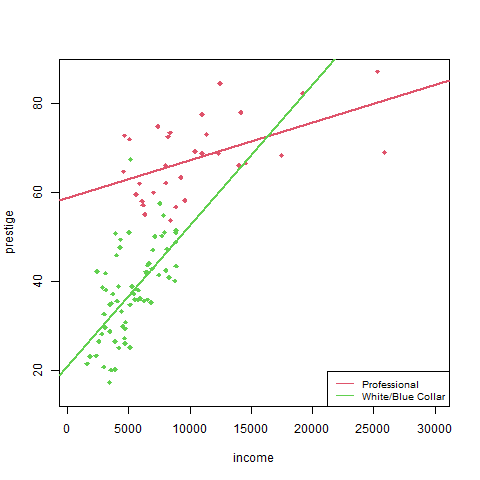
\includegraphics[width=0.9\textwidth]{Graphics/prestige_interaction.png}
		    \caption{Prestige as a function of income, professional job type and their interaction}
		    \label{fig:pres_inc_prof}
	    \end{figure}

\clearpage

	\item [(c)] \textbf{Prediction Equation}:

    if y = prestige, x = income, z = professional
\begin{equation}\label{eq:pred}
    \hat{y}  =  \beta_0 + \delta_1 z + \beta_1x +\delta_2 xz + \epsilon
\end{equation}
\[ \beta_0 = 21.14226, \beta_1 = 0.003171, \delta_1 = 37.78128, \delta_2 = -0.002326\]

  ie
  
    $prestige =
      21.14226 + 37.78128\times professional + 0.003171\times income +
      (-0.002326)\times professional\times income$


\begin{comment}
https://imaging.mrc-cbu.cam.ac.uk/statswiki/FAQ/contint?action=AttachFile&do=get&target=int.pdf
\end{comment}

%\newpage
	\item [(d)] 	%Interpret 
	The coefficient for \texttt{income} is $\beta_1 +\delta_2 z = 0.003171 -0.002326\times professional$ 
	
	Assuming professional status is constant, a \$1 rise in \texttt{income} results in a predicted rise in prestige of 0.003171 if in a blue collar or white collar job; prestige rises by 0.000845 per \$ (ie 0.003171-0.002326) if in a professional job.
	
	\item [(e)] %Interpret the coefficient for \texttt{professional}. 
	The coefficient for \texttt{professional} is $\delta_1  + \delta_2 x =  37.78128-0.002326\times income$
	
  If \texttt{professional} switches to $1$ (ie \texttt{type = prof}) then \texttt{prestige} increases by 37.78128 -0.002326$\times$ \texttt{income}, if \texttt{income} is held constant.
  If \texttt{professional} changes to $1$ and \texttt{income} changes, the change in prestige is 37.78128 - 0.002326 $\times$ old income + 0.000845 $\times$ change in \texttt{income}.
	
	\item [(f)]
%	What is the effect of a \$1,000 increase in income on prestige score for professional occupations? In other words, we are interested in the marginal effect of income when the variable \texttt{professional} takes the value of $1$. Calculate the change in $\hat{y}$ associated with a \$1,000 increase in income based on your answer for (c).
	
	If \texttt{professional} = 1, and $\Delta income = 1000$ then the equation becomes 
  \[\Delta\hat{y} = ((\beta_1 +\delta_2\times 1)\times  1000 \]

  The marginal effect on \texttt{prestige} of an increase of \$1,000 in income, for professional occupations:  
  $ = (0.003171-0.002326)\times 1000 = 0.845$
  
	\item [(g)]
%	What is the effect of changing one's occupations from non-professional to professional when her income is \$6,000? We are interested in the marginal effect of professional jobs when the variable \texttt{income} takes the value of $6,000$. Calculate the change in $\hat{y}$ based on your answer for (c).
%        (Intercept)              income        professional income:professional 
%       1.142258854         0.003170909        37.781279955        -0.002325709 
	From equation~\ref{eq:pred}, if \texttt{income} $x$ is 6000, then when \texttt{professional} $z_0$ was 0, \texttt{prestige} was:

  \[\hat{y_0} = (\beta_0) + (\beta_1) x = 21.14226 + 0.003171\times 6000 = 40.16826\]
	
	when \texttt{professional} $z_1$ is 1, \texttt{prestige} is:
  \[\hat{y}_1  = (\beta_0 + \delta_1) + (\beta_1 +\delta_2) x z_1 \]
      
      \[= (21.14226 + 37.78128) + (0.003171-0.002326)*6000 = 63.99354  \]
	
  so, \[\Delta\hat{y} = \hat{y}_1 - \hat{y}_0 = 63.99354 - 40.16826 = 23.82528 \]

	(or, $\Delta\hat{y}  =  \delta_1 + \delta_2 x = 37.78128-0.002326\times 6000 $)
  
  The marginal effect of professional jobs when the variable \texttt{income} takes the value of \$6,000 is an increase in \texttt{prestige} of 23.82528.
  
\end{enumerate}

\newpage

\section*{Question 2: Political Science}
%\vspace{.25cm}
\noindent 	Researchers are interested in learning the effect of all of those yard signs on voting preferences.\footnote{Donald P. Green, Jonathan	S. Krasno, Alexander Coppock, Benjamin D. Farrer,	Brandon Lenoir, Joshua N. Zingher. 2016. ``The effects of lawn signs on vote outcomes: Results from four randomized field experiments.'' Electoral Studies 41: 143-150. } Working with a campaign in Fairfax County, Virginia, 131 precincts were randomly divided into a treatment and control group. In 30 precincts, signs were posted around the precinct that read, ``For Sale: Terry McAuliffe. Don't Sellout Virgina on November 5.'' \\

Below is the result of a regression with two variables and a constant.  The dependent variable is the proportion of the vote that went to McAuliff's opponent Ken Cuccinelli. The first variable indicates whether a precinct was randomly assigned to have the sign against McAuliffe posted. The second variable indicates
a precinct that was adjacent to a precinct in the treatment group (since people in those precincts might be exposed to the signs).  \\

\vspace{.5cm}
\begin{table}[!htbp]
	\centering 
	\textbf{Impact of lawn signs on vote share}\\
	\begin{tabular}{@{\extracolsep{5pt}}lccc} 
		\\[-1.8ex] 
		\hline \\[-1.8ex]
		Precinct assigned lawn signs  (n=30)  & 0.042\\
		& (0.016) \\
		Precinct adjacent to lawn signs (n=76) & 0.042 \\
		&  (0.013) \\
		Constant  & 0.302\\
		& (0.011)
		\\
		\hline \\
	\end{tabular}\\
	\footnotesize{\textit{Notes:} $R^2$=0.094, N=131}
\end{table}

  \begin{lstlisting}
  n <- 131
  est_coeffs <- 3
  df <- n - est_coeffs
  R2 <- 0.094
  \end{lstlisting}

%\vspace{.5cm}
\begin{enumerate}
	\item [(a)] To determine whether having these yard signs in a precinct affects vote share we conduct a hypothesis test with $\alpha = .05$.  The null hypothesis is that having yard signs in a precinct have no effect on the voting in that precinct, ie $H_0: \beta_1 = 0, H_{alt}: \beta_1 \ne 0$.  

  \begin{lstlisting}
    beta1 <- 0.042
    n1 <- 30
    se1 <- 0.016

    t_precinct <- beta1 / se1
    pval_precinct <- 2*pt(abs(t_precinct), df, lower.tail=FALSE)
  \end{lstlisting}
  
	$tvalue =  0.042/0.016 = 2.625$
	
	$pvalue =  Pr(tvalue = 2.625, df = 128) = 0.00972002$
	
  $pvalue < \alpha$, so we reject the null hypothesis and conclude that the presence of signs in yards in a precinct is associated with an average increase in vote for Cuccinelli of 4.2\% in that precinct.

	\item [(b)]  To determine whether being
	next to precincts with these yard signs affects vote
	share we conduct a hypothesis test with $\alpha = .05$. The null hypothesis is that having yard signs in a precinct have no effect on the voting in the adjacent precincta, ie $H_0: \beta_2 = 0, H_{alt}: \beta_2 \ne 0$. 
	
  \begin{lstlisting}
    n2 <- 76
    beta2 <- 0.042
    se2 <- 0.013

    t_adj <- beta2 / se2
    pval_adj <- 2*pt(abs(t_adj), df, lower.tail = FALSE)
  \end{lstlisting}

	$tvalue =  0.042/0.013 = 3.230769$
	
	$pvalue = 0.00156946$
	
  $pvalue < \alpha$, so we reject the null hypothesis and conclude that the presence of signs in yards in a precinct is associated with an average increase in vote for Cuccinelli of 4.2\% in the adjacent precincts.	
  
	\item [(c)] %Interpret the coefficient for the constant term substantively.
	If not in a precinct with yard signs and not in an adjacent precinct, Cuccinelli averages 30.2\% of the vote.
	
	At the 95\% confidence level, the vote for Cuccinelli in a precinct which is considered
	to be unaffected by signs is between  28.02\% and 32.38\%. 

	\begin{lstlisting}
    beta0 <- 0.302
    se0 <- 0.011

  	tscore <- qt(0.975, df) # get tscore for df 128,

    CI0_L <- beta0 - tscore*se0
    CI0_U <- beta0 + tscore*se0
	\end{lstlisting}
    
  t-statistic for two-sided test with $\alpha = 0.95\%$, 128 degrees of freedom = 1.978671

	\item [(d)] %Evaluate the model fit for this regression.  What does this	tell us about the importance of yard signs versus other factors that are not modeled?

\begin{comment}
  The assumptions for this model are:	
  \begin{itemize}
  \item Linear relationships between Y and X1, Y and X2.
  \item Independent covariates
  \item 0 conditional mean (errors average 0 for any value of X)
  \item Equal variance for all i (in expectation), and uncorrelated
  \item X is unrelated to e
  \end{itemize}
\end{comment}
  If the assumptions are valid, the presence of yard signs (even if they don't mention the candidate or their party) can predict an increase in votes of 4.2\%\footnote{CI $\beta_1$: 1.03\% to 7.37\%;  CI $\beta_2$: 1.63\% to 6.77\%, at 95\%}.  That could be the difference between winning an losing a close election, so the signs would be worth the cost, particularly as they increased vote share in 106 precincts, even though they were only placed in 30.

The model's value is based on the test being set up with a effectively random/representative assignment of yard signs (it couldn't be actually random, or there would have been precincts with yard signs adjacent to each other).  This assumes precincts are homogeneous with regard to party affiliation, voter turnout, through traffic, size (affecting proportion of voters who would have seen the signs), etc.

The model assumes predictors are independent, ie that the vote share in the adjacent precincts is not being affected by some other characteristic based on proximity to the areas with yard signs, and that the change in vote share is not due to a confounding variable which affects the sign and adjacent precincts, but which is not being modelled.


  However, the $R^2$ value is 0.094, ie only 9.4\% of the variation in the dependent variable can be explained by the yard sign model.  Most of the variation in vote share results from factors which are not modelled.  If those missing variables were accounted for they could change both the values and the significance of the coefficients.   Alternatively, the relationship between the dependent variable (vote share) and the predictors (yard signs) may not be linear, and an alternative model, with the same predictors, might be appropriate.

  
\end{enumerate}  

\newpage
\section{Appendix}
  \subsubsection{Code}
  \verb|PS04_ImeldaFinn.R|
  
  
  \subsubsection*{Q1 - model variations depending on treatment of missing values}
  
  Went with conservative option of ignoring NAs rather than recoding.  
  The difference to the coefficients and p-values wasn't significant.
	 \lstinputlisting[language=R, firstline=136, lastline=147]{PS04_ImeldaFinn.R}


  
% Table created by stargazer v.5.2.3 by Marek Hlavac, Social Policy Institute. E-mail: marek.hlavac at gmail.com
% Date and time: Thu, Dec 01, 2022 - 02:32:39
\begin{table}[!htbp] \centering 
  \caption{Effect of na job types on model} 
  \label{tab:pres_nas} 
\begin{tabular}{@{\extracolsep{5pt}}lccc} 
\\[-1.8ex]\hline 
\hline \\[-1.8ex] 
 & \multicolumn{3}{c}{\textit{Dependent variable:}} \\ 
\cline{2-4} 
\\[-1.8ex] & \multicolumn{3}{c}{prestige} \\ 
\\[-1.8ex] & (1) & (2) & (3)\\ 
\hline \\[-1.8ex] 
 income & 0.0032$^{***}$ & 0.0033$^{***}$ & 0.0032$^{***}$ \\ 
  & (0.0005) & (0.0005) & (0.0005) \\ 
  & & & \\ 
 professional & 37.7813$^{***}$ & 38.1200$^{***}$ & 37.1860$^{***}$ \\ 
  & (4.2483) & (4.0798) & (4.0920) \\ 
  & & & \\ 
 income:professional & $-$0.0023$^{***}$ & $-$0.0024$^{***}$ & $-$0.0023$^{***}$ \\ 
  & (0.0006) & (0.0005) & (0.0005) \\ 
  & & & \\ 
 Constant & 21.1423$^{***}$ & 20.8035$^{***}$ & 21.0533$^{***}$ \\ 
  & (2.8044) & (2.5387) & (2.5748) \\ 
  & & & \\ 
\hline \\[-1.8ex] 
Observations & 98 & 102 & 102 \\ 
R$^{2}$ & 0.7872 & 0.7893 & 0.7863 \\ 
Adjusted R$^{2}$ & 0.7804 & 0.7828 & 0.7797 \\ 
Residual Std. Error & 8.0116 (df = 94) & 8.0181 (df = 98) & 8.0747 (df = 98) \\ 
F Statistic & 115.8778$^{***}$ (df = 3; 94) & 122.3380$^{***}$ (df = 3; 98) & 120.1705$^{***}$ (df = 3; 98) \\ 
\hline 
\hline \\[-1.8ex] 
\textit{Note:}  & \multicolumn{3}{r}{$^{*}$p$<$0.1; $^{**}$p$<$0.05; $^{***}$p$<$0.01} \\ 
\end{tabular} 
\end{table}  


  \subsubsection*{Q2}

	A full F-test was used to evaluate hypothesis that all the coefficients are 0; at 5\% reject null hypothesis.
	
	\begin{lstlisting}
  	F.test <-(R2/(k-1))/((1-R2)/(n-k))
    #F test statistic F = 6.640 with 2 and 129 degrees of freedom
    df1 <- k - 1
    df2 <- n-k

    F.pvalue <-df(F.test, df1, df2)
    # 0.001634304
	\end{lstlisting}
\end{document}
